\subsubsection{Opis przypadków użycia - zamówienia}

Przypadki użycia wyjaśniające funkcjonalności systemu związane z zarządzaniem
zamówieniami.

\begin{figure}[h!]
    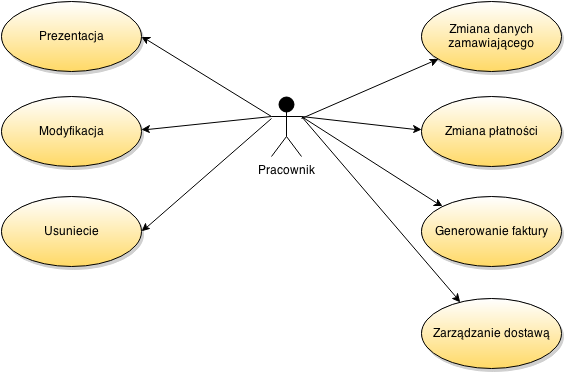
\includegraphics[width=\textwidth,
    height=0.5\textheight]{graphics/UseCase/Zamowienia/UseCaseDiagram.png}
  \caption{Diagram przypadków użycia związanych z procesowaniem zamówień}
\end{figure}

\begin{enumerate}
  \item Prezentacja zamówień\\
  \begin{tabularx}{\linewidth}{ c X }
  Aktor: & Pracownik \\
  Opis: & Prezentacja panelu z listą wszystkich zamówień znajdujących się w~systemie
  oraz możliwościami kontroli i zarządzania nimi.\\
  \end{tabularx}
	\begin{enumerate}
	  \item Pracownik loguje się w Panelu Zarządzania
	  \item Wybiera Panel Zarządzania Zamówieniami
	  \item Wyświetlana jest lista zamówień z możliwością modyfikacji widoków
	  oraz panelem opcji (wszystkie opisane w poniższych przypadkach użycia)
	\end{enumerate}

  \item Edycja, modyfikacja zamówień\\
  \begin{tabularx}{\linewidth}{c X}
  Aktor: & Pracownik \\
  Opis: & Funkcjonalność umożliwia modyfikację produktów w zamówieniu oraz
  zmianę danych odbiorcy.
  \end{tabularx}
	\begin{enumerate}
	  \item Pracownik po autoryzacji w panelu sterowania systemu, przechodzi do
	  panelu Zarządzania Zamówieniami (patrz Zamowienia przypadek użycia 1)
	  \item Z wyświetlonej przez system listy zamówień, pracownik wybiera jeden
	  element
	  \item W celu edycji produktów:
		\begin{enumerate}
		  \item Wybiera opcję podglądu zawartości zamówienia
		  \item Z wyświetlonej listy zamówionych produktów zaznacza jedną pozycję
		  \item Wybiera opcję edycji
		  \item Otrzymuje informacje o konkretnym produkcie (jego ID, szczegółowy opis)
		  oraz zamówioną ilość oraz podsumowanie (cenę, informację o udzielonych rabatach na dany produkt)
		  \item Pole z ilością produktu umożliwia modyfikację – wystarczy wprowadzić
		  liczbę z zakresu od 1 do maksymalnej liczby aktualnie dostępnych produktów w
		  magazynie (0 nie wchodzi w zakres bo do tego służy funkcja usunięcia)
		\end{enumerate}
	  \item W celu usunięcia produktu:
		\begin{enumerate}
		  \item Wybiera opcję podglądu zawartości zamówienia
		  \item Z wyświetlonej listy zamówionych produktów zaznacza jedną pozycję
		  \item Wybiera opcję Usuń
		  \item System pyta o potwierdzenie i po akceptacji dokonuje wykluczenia
		  produktu z zamówienia oraz wysyła powiadomienie do Zamawiającego
		\end{enumerate}
	  \item W celu dodania produktu:
		\begin{enumerate}
		  \item Wybiera opcję podglądu zawartości zamówienia
		  \item Wybiera opcję Dodaj produkt
		  \item Otworzony zostaje system zakupowy\\ 
		  (przebieg wyboru produktu - opisany w przypadkach użycia odnoszących się do
		  Produktów)
		  \item Po wybraniu produktu system wyświetla informację o tym jakie zostaną
		  wprowadzone zmiany i czeka na akceptację
		  \item Po akceptacji, zamówienie zostaje zmodyfikowane (produkt dodany),
		  koszt zaktualizowany oraz system informuje odbiorcę zamówienia (klienta) o
		  zaszłych zmianach – za pomocą wiadomości email (z ewentualną poprawioną
		  fakturą pro-forma, jeśli była zaznaczona taka opcja) 
	  \end{enumerate} %koniec alternatywy Dodania produktu
	\end{enumerate} %koniec UC Edycja, modyfikacja zamówień
  
  \item Zmiana danych zamawiającego\\
  \begin{tabularx}{\linewidth}{c X}
  Aktor: & Pracownik \\
  Opis: & Można zmienić dane odbiorcy na potrzeby danego zamówienia (zmiana
  danych tylko w ramach konkretnej faktury). Dotyczy to w szczególności adresu i
  danych osobowych osoby odpowiedzialnej za zamówienie.
  \end{tabularx}  
	\begin{enumerate}
	  \item Pracownik po autoryzacji w panelu sterowania systemu, przechodzi do
	  panelu Zarządzania Zamówieniami (patrz Zamówienia przypadek użycia 1)
	  \item Z wyświetlonej przez system listy zamówień, pracownik wybiera jeden
	  element i wybiera opcję Zmień Dane Odbiorcy
	  \item System prezentuje aktualnie dane odbiorcy (mogą to być aktualne dane
	  klienta, albo już wcześniej modyfikowane dane osobowe wprowadzone specjalnie w
	  ramach tego zamówienia)
	  \item Pracownik modyfikuje wybraną przez siebie składową danych (wszystkie
	  elementy pozwalają na edycję) i zatwierdza wprowadzone zmiany
	  \item System wyświetla zapytanie o potwierdzenie zmian i po jego akceptacji
	  wysyła powiadomienie do klienta o zaszłych zmianach – wiadomość drogą
	  elektroniczną
	\end{enumerate}

  \item Usunięcie zamówienia w całości\\
  \begin{tabularx}{\linewidth}{c X}
  Aktor: & Pracownik \\
  Opis: & Istnieje możliwość anulowania zamówienia – na życzenie klienta lub z
  powodów biznesowych sklepu.
  \end{tabularx}  
	\begin{enumerate}
	  \item Pracownik po autoryzacji w panelu sterowania systemu, przechodzi do
	  panelu Zarządzania Zamówieniami (patrz Zamówienia przypadek użycia 1)
	  \item Z wyświetlonej przez system listy zamówień, pracownik wybiera jeden
	  element i wybiera opcję Usuń zamówienie
	  \item System wyświetla ostrzeżenie (wraz ze szczegółową informacją o
	  zamówieniu) i pyta o potwierdzenie
	  \item Pracownik potwierdza chęć usunięcia danego zamówienia. Ma też możliwość
	  wpisania krótkiego uzasadnienia tej operacji
	  \item System dokonuje usunięcia oraz wysyła powiadomienie o anulowaniu
	  zamówienia do zamawiającego (drogą elektroniczną)
	\end{enumerate}

  \item Edycja formy płatności\\
  \begin{tabularx}{\linewidth}{c X}
  Aktor: & Pracownik \\
  Opis: & Pracownik ma możliwość zmiany początkowo wybranej formy płatności
  danego zamówienia. Odbywa się to na wniosek zamawiającego lub osoby
  odpowiedzialnej za zamówienia po stronie Sklepu.
  \end{tabularx}    
	\begin{enumerate}
	  \item Z listy zamówień pracownik wybiera jedno i wybiera opcję Zmiana formy
	  płatności
	  \item System prezentuje widok wyboru pomiędzy dostępnymi formami płatności
	  (specyfikacja w wymaganiach niefunkcjonalnych punkt \ref{itm:Platnosci})
	  \item Pracownik dokonuje wyboru formy oraz waluty.
	  \item System powiadamia klienta o zmianie formy płatności drogą elektroniczną.
	\end{enumerate}

  \item Wybór sposobu potwierdzenia zamówienia\\
  \begin{tabularx}{\linewidth}{c X}
  Aktor: & Pracownik \\
  Opis: & Możliwość zmiany sposobu udokumentowania przeprowadzonej transakcji
  (zazwyczaj będzie to faktura albo paragon). Powodem takich zmian mogą być
  nawet regulacje prawne.
  \end{tabularx}	
	\begin{enumerate}
	  \item Z listy zamówień pracownik wybiera jedno i wybiera opcję Zmiana
	  Potwierdzenia Transakcji
	  \item System prezentuje widok wyboru pomiędzy dostępnymi sposobami
	  potwierdzenia (udokumentowania) prowadzonej transakcji (wymagania
	  niefunkcyjne punkt \ref{itm:PotwierdzenieTransakcji})
	  \item Pracownik dokonuje wyboru oraz może uruchomić proces generacji
	  dokumentu.
	  \item W przypadku generacji dokumenty system wyświetla go pracownikowi.
	  \item Po akceptacji informacje o zmianie wraz z dokumentami wysyłane są drogą
	  elektroniczną do klienta.
	\end{enumerate}

  \item Generowanie faktury pro-forma dla danego zmówienia\\
  \begin{tabularx}{\linewidth}{c X}
  Aktor: & Pracownik \\
  Opis: & Możliwość utworzenie faktury pro-forma na podstawie danego zamówienia
  oraz przesłanie jej klientowi drogą elektroniczną lub wydruk.
  \end{tabularx}
	\begin{enumerate}
	  \item Z listy zamówień pracownik wybiera jedno i wybiera opcję Generuj
	  Pro-Forma
	  \item Dla wybranego zamówienia system generuje pełną fakturę po czym
	  prezentuje ją pracownikowi
	  \item Pracownik ma możliwość odrzucenia lub akceptacji dokumentu.
	  \item W przypadku akceptacji system wyświetla widok wyboru z opcjami wysyłki
	  do klienta.
	  \item Po wybraniu pożądanej opcji przez pracownika, system wysyła dokument do
	  klienta albo do drukarki.
	\end{enumerate}

  \item Zarządzanie dostawą\\
  \begin{tabularx}{\linewidth}{c X}
  Aktor: & Pracownik \\
  Opis: & Termin realizacji zamówienia oraz sposób dostawy mogą być
  modyfikowany dowolnie w zależności od możliwości biznesowych Sklepu i
  aktualnego stanu zamówienia.
  \end{tabularx}
	\begin{enumerate}
	  \item Z listy zamówień użytkownik wybiera jedno i wybiera opcję Edycji
	  Dostawy
	  \item System prezentuje informacje o wybranym sposobie i terminie dostawy
	  \item Użytkownik wybiera opcję Zmiany daty realizacji
	  \item System prezentuje widok kalendarza z zaznaczoną dotychczasową datą
	  realizacji.
	  \item Użytkownik przesuwa datę realizacji projektu i ma możliwość podania
	  wiadomości wyjaśniającej modyfikację.
	  \item Użytkownik wybiera opcję Zmiany sposobu dostawy
	  \item System wyświetla wszystkie aktualnie dostępne opcje razem ze
	  szczegółami (cena, średni czas)
	  \item Użytkownik dokonuje wyboru środka transportu i zatwierdza zmiany
	  \item System aktualizuje koszt całego zamówienia uwzględniając kwotę
	  transportu oraz wysyła powiadomienie o zmianach (termin lub/i sposób dostawy)
	  do klienta wraz z informacją wyjaśniającą wpisaną przez pracownika.
	\end{enumerate}

  \item Ustawianie aktualnego stanu zamówienia\\
  \begin{tabularx}{\linewidth}{c X}
  Aktor: & Pracownik \\
  Opis: & Zamówienie może znajdować się w pewnych stanach realizacji (np. w
  przygotowaniu, w realizacji, wysłane - konkretne stany określają wymagania
  niefunkcjonalne). Istnieje możliwość zmiany aktualnego stanu zamówienia.
  \end{tabularx}
	\begin{enumerate}
	  \item Z listy zamówień pracownik wybiera jedno i wybiera opcję Zmień Stan
	  \item System prezentuje widok z dostępnymi stanami dla danego zamówienia
	  \item Pracownik dokonuje wyboru i zatwierdza zmiany.
	  \item Jeśli pracownik wybiera opcję Powiadom, to system powiadamia klienta o
	  zmianie stanu jaka nastąpiła i przesyła krótkie wyjaśnienie.
	\end{enumerate}
	 
\end{enumerate}
